\title{Expectation Maximization}
\label{chp:label}
\author{Bruno Almeida Pimentel}
\institute{Instituto de Computação - Universidade Federal de Alagoas}

\maketitle


%\chapter{Optimization}

Expectation Maximization (or also known as EM) is one of the algorithms most frequently used in Machine Learning \cite{moon1996expectation, do2008expectation}. This popularity is due to its algorithm simplicity. EM is used in various applications, such as Data Mining, Clustering, Natural Language Processing, Signal Processing,  medical image reconstruction and others \cite{dellaert2002expectation, dempster1977maximum, ceppellini1955estimation, tzoreff2017expectation, li2019expectation}.

This chapter is divided as follows. Section \ref{sec:coin} shows an experiment with coin-flipping in order to better understand the mathematical behinds the EM algorithms. Section \ref{sec:math} shows the mathematical foundations of EM. Section \ref{sec:algorithm} concerns about the algorithm. And Section \ref{sec:applications} presents where EM algorithms can be used in real applications. 

\section{A coin-flipping experiment}
\label{sec:coin}

In order to better understand the mathematical foundations and the process behind the Expectation Maximization algorithm, this section concerns about a simple experiment with coin-flipping. For this, suppose that we want to estimate the bias of two coins. Also, consider that these coins can be fair or not (i.e. they can be more heavily weighted towards heads). This experiment is based on steps where each one has two main actions:

\begin{itemize}
    \item Randomly choose a coin;
    \item Flip the chosen coin $10$ times.
\end{itemize}

After carrying out these steps $6$ times, we can achieve this table:

\begin{center}
\begin{tabular}{|c|c|c|c|c|} 
 \hline
 \textbf{Steps} &\textbf{Coin} & \textbf{Flips} & \textbf{\# coin A heads} & \textbf{\# coin B heads} \\ \hline 
1 & A & HTTTHHTHTH & 5 & 0\\ \hline 
2 & B & HHHHTHHHHH & 0 & 9\\ \hline
3 & B & HTHHHHHTHH	& 0 & 8\\ \hline 
4 & B & HTHTTTHHTT & 0 & 4\\ \hline
5 & A & THHHTHHHTH & 7 & 0\\ \hline 
6 & B & HTTHTHHHHH & 0 & 7\\ \hline
\end{tabular}
\end{center}

To estimate each coin's bias independently, we would consider the total of heads and the total of flips. For coin A, the total of flips is equal to $20$ ($2$ trials and $10$ flips each one). Thus, the bias of coin A would be 12/20. Similarly, for coin B, its bias would be 28/40. Therefore, when we know which coin is flipped, the problem of estimating the coin's bias can be solved as above. However, what about if we not know which coin is flipped?

When we do not know which coin is flipped, our table can be rewritten as follows:

\begin{center}
\begin{tabular}{|c|c|c|c|c|} 
 \hline
 \textbf{Steps} & \textbf{Coin} & \textbf{Flips} & \textbf{\# coin A heads} & \textbf{\# coin B heads} \\ \hline 
1 & ? & HTTTHHTHTH & ? & ?\\ \hline 
2 & ? & HHHHTHHHHH & ? & ?\\ \hline
3 & ? & HTHHHHHTHH	& ? & ?\\ \hline 
4 & ? & HTHTTTHHTT & ? & ?\\ \hline
5 & ? & THHHTHHHTH & ? & ?\\ \hline 
6 & ? & HTTHTHHHHH & ? & ?\\ \hline
\end{tabular}
\end{center}

This means that we do not know about the target variable (coin A or B). In this context, EM algorithm can be used to estimate the bias of each coin. For this, the EM algorithm starts guessing a solution; that is, it starts with a guess for the coin's biases. From this initial guess, we are able to estimate which coin was chosen in each trial. Then, based on each trial, we can calculate the number of heads for each coin among the trials (this step is called the E-step in the EM algorithm). From this number of heads estimated in the previous step, we can calculate a better guess for the bias of each coin (M-step). This process of alternation between E-step and M-step is carried out until no significant modification in the value of each coin's bias is achieved. The next sections show more details of mathematical foundations and how the algorithm works step by step.

\section{Mathematical foundations}
\label{sec:math}

Let $\textbf{X} = \{\textbf{x}_1,\ldots, \textbf{x}_i,\ldots, \textbf{x}_N\}$ be the data set which consists of N observed samples and each data point $\textbf{x}_i$ has its corresponding latent variable $\textbf{z}_i$.  Let $\{\textbf{X}, \textbf{Z}\}$ be the complete data and its log-likelihood function takes the form $ln \text{ }p (\textbf{X}, \textbf{Z}|\theta)$, where $\theta$ is the set of all parameters of the model. In practice, the only knowledge of latent variables in $\textbf{Z}$ is given by the posterior distribution $p (\textbf{Z}|\textbf{X}, \theta)$. 

The EM algorithm aims to maximize the likelihood
$ln \text{ }p (\textbf{X}, \textbf{Z}|\theta)$ by two mains steps: E step and the M step. In the E step, we use the current parameters, here called $\theta^{old}$, to find the posterior distribution of $\textbf{Z}$ given by $p (\textbf{Z}|\textbf{X}, \theta)$. Then we use the posterior distribution to find the expectation of the complete data likelihood $Q(\theta, \theta^{old})$, computed as following:

\begin{equation}
    Q(\theta, \theta^{old}) = \sum_{\textbf{z}} p(\textbf{Z}|\textbf{X},\theta^{old}) ln \text{ } p(\textbf{X}, \textbf{Z}|\theta)
\end{equation}

Then in the M step, the revised parameter $\theta^{new}$ is determined by maximizing the function:

\begin{equation}
    \theta^{new} = \underset{\theta}{\mathrm{arg max }} Q(\theta, \theta^{old})
\end{equation}

The E and M steps are executed alternatively until the convergence of the algorithm. Details about these steps and convergence criterion are discussed in Section \ref{sec:algorithm}. 

\subsection{Gaussian Mixture}

Gaussian Mixture Model (abbreviated as GMM) \cite{richardson1997bayesian} can be understood as an special case of EM algorithm. A mixture model is based on combination of multiple probability distribution functions. GMM algorithm uses a combination of Gaussian (or Normal $N$) probability distributions. On the other hand, GMM needs to estimate the mean ($\bm{\mu}$) and standard deviation (from $\bm{\Sigma}$) parameters for each Gaussian. Therefore, the posterior distribution $p$ can be rewritten using the Normal distribution as following: 

\begin{equation}
    p(\textbf{x}_i) = \sum_{k=1}^K z_{ik} N(\textbf{x}_i| \bm{\mu}_k, \bm{\Sigma}_k).
\end{equation}

Then the likelihood function is given as the expression:

\begin{equation}
    ln \text{ } p(\textbf{X}, \textbf{Z}|\bm{\mu}, \bm{\Sigma}) = \sum_{i=1}^N \left[ \sum_{k=1}^K z_{ik} N(\textbf{x}_i| \bm{\mu}_k, \bm{\Sigma}_k) \right].
\end{equation}

The value of $z_{ik}$ follows the restriction: $\sum_{k=1}^K z_{ik}=1$. This can be interpreted as the influence (weight) of each distribution takes to sample $\textbf{x}_i$. After some algebra, the value of $z_{ik}$ that satisfies the restriction is computed in the E step of GMM algorithm as following:

\begin{equation}
    z_{ik}^{new} = \frac{N(x_i|\bm{\mu}_k^{new}, \bm{\Sigma}_k)}{\sum_{k=1}^K N(x_i|\bm{\mu}_j^{new}, \bm{\Sigma}_j)}.
\label{z_new}
\end{equation}

In the M step, the parameters $\bm{\mu}$ and $\bm{\Sigma}$ of Normal probability distribution are computed using the expressions:

\begin{equation}
    \bm{\mu}_k^{new} = \frac{1}{N_k} \sum_{i=1}^N z_{ik}^{new} \textbf{x}_i,
\label{mu_new}
\end{equation}

\begin{equation}
    \bm{\Sigma}_k^{new} = \frac{1}{N_k} \sum_{i=1}^N z_{ik}^{new} (\textbf{x}_i-\bm{\mu}_k^{old})(\textbf{x}_i-\bm{\mu}_k^{old})^T,
\label{sigma_new}
\end{equation}

\noindent where $N_k$ is given as:

\begin{equation}
    N_k = \sum_{i=1}^N z_{ik}^{new}.
\end{equation}

After the convergence of GMM algorithm, i.e., when parameters achieve a stationary value, the estimated $\textbf{x}_i^{new}$ is computed as:

\begin{equation}
    \textbf{x}_i^{new} = \sum_{i=1}^N z_{ik}^{new} \bm{\mu}_k^{new}
\end{equation}

Figure \ref{example_mixture} shows an example of Gaussian mixture from three Normal distribution. The mean parameter of the Normal distributions are, respectively, $5$, $10$ and $17$; the three Normal distributions have standard deviations equal to $2$. Dotted lines indicate the respective Normal distribution and the continuous line shows the density of these distributions. Each distribution has equal weight (1/3). 

\begin{figure}[ht]
\centering
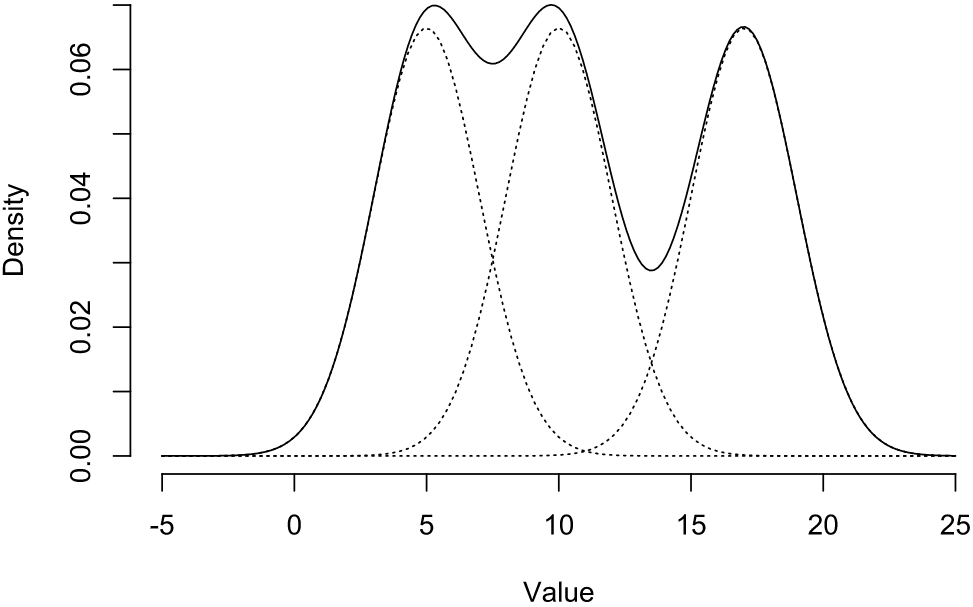
\includegraphics[width=11cm]{Part 3 - Learning Systems/Unsupervised Learning/Expectation-Maximization/figures/gaussian_mixture.png}
\caption{Example of Gaussian mixture. Adapted from \cite{Smason79}.}
\label{example_mixture}
\end{figure}

\subsection{Example}

The covariance matrix $\bm{\Sigma}$ gives the algorithm the ability to identify clusters of different shapes and sizes. The diagonal values of the matrix are the variance of a given variable: the bigger this value, the more spread out the cluster is. Values that outsize the diagonal quantifies the covariance between pairs of variables. From covariance value, the correlation between variables can be computed.

In order to illustrate the importance of covariance matrix $\bm{\Sigma}$, Figure \ref{example_partition} shows an example of a simple data set and resulting partitions after applying the well known K-Means algorithm and the EM algorithm for the spacial case when $\bm{\Sigma}$ is a diagonal matrix. 

\begin{figure}[ht]
\centering
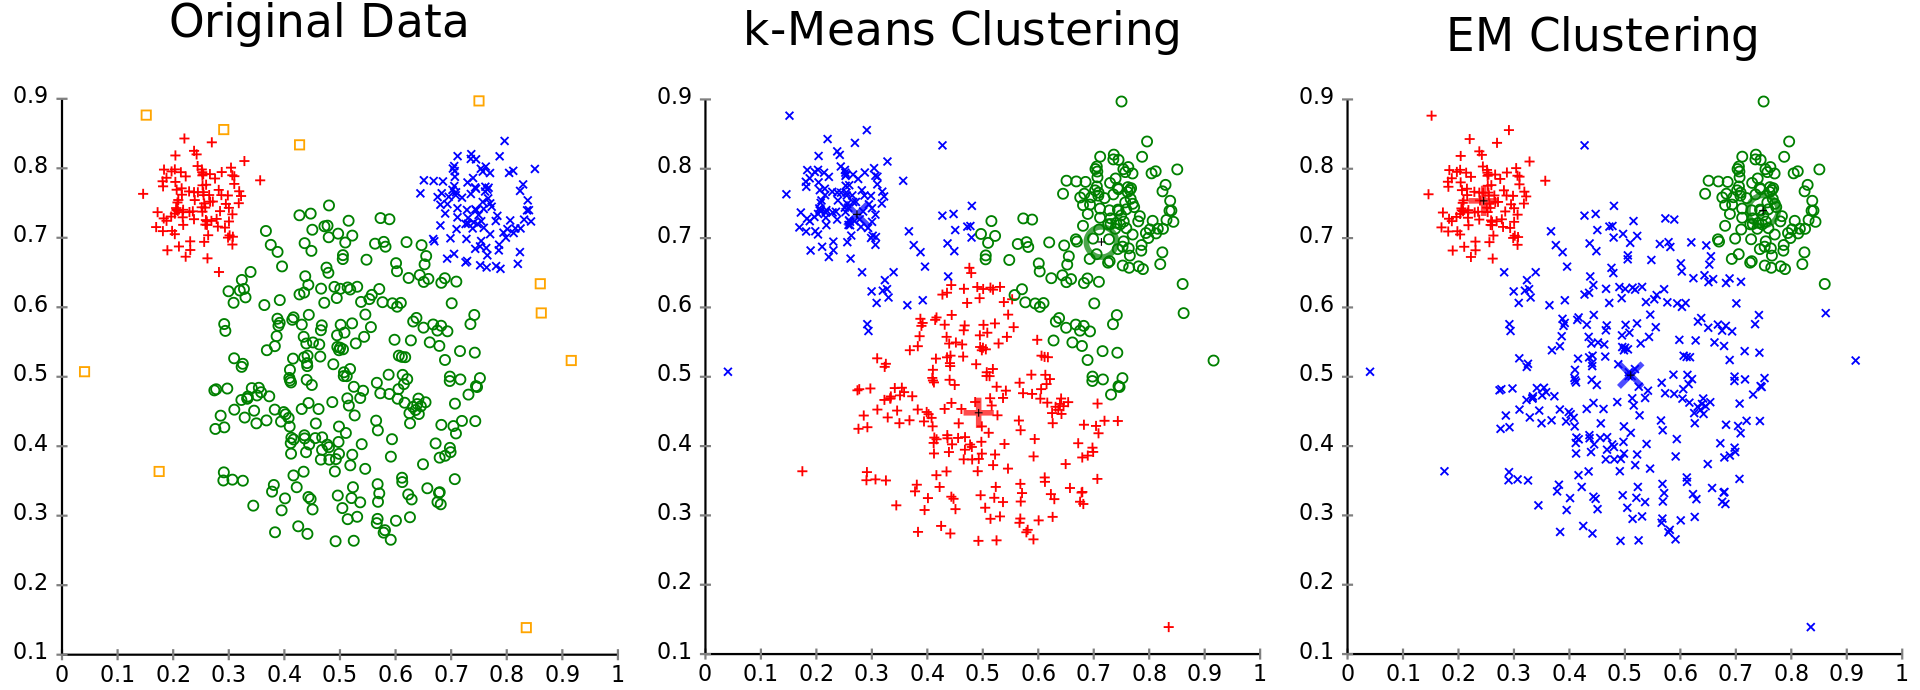
\includegraphics[width=13cm]{Part 3 - Learning Systems/Unsupervised Learning/Expectation-Maximization/figures/ClusterAnalysis_Mouse.png}
\caption{Example of partitions found by K-Means and EM clustering algorithms. Adapted from \cite{Chire}.}
\label{example_partition}
\end{figure}

The original data set contains three classes with different spherical sizes. After applying K-Means clustering algorithm, the resulting partition is different from original one since this algorithm divides the space into clusters of equal dispersion. In other words, K-Means intends to find spherical clusters of equal sizes. On the other hand, after applying EM algorithm, the resulting partition is similar to original one. This is because EM algorithm is able to create a model that identifies different distributions, which allows to find a resulting partition with clusters of different sizes and shapes.

\section{Algorithm}
\label{sec:algorithm}

EM is broadly used in Machine Leaning applications because EM algorithm is simple and easy to understand. Algorithm \ref{pseudocod} shows the main steps.

%%%%%%%%%%%%%%%%%%%%%%%% ALGORITHM
\begin{algorithm}[ht]
	%\renewcommand{\baselinestretch}{0.8}
	\caption{EM algorithm}
	\label{pseudocod}
    
    Parameters: Data set $\textbf{X}$, number of cluster $K$.
    
    Output: Final partition.
    
	\begin{algorithmic}[1] 
		\STATE{Choose initial parameters. Set $t=0$. Set $\epsilon$.}
		
        \REPEAT
		
		\STATE \textbf{E-step}: update the value of $z_{ik}^{new}$ using the Equation \ref{z_new}, under the restriction $\sum_{k=1}^K z_{ik}=1$.
		
		\STATE \textbf{M-step}: update the parameters $\bm{\mu}_k^{new}$ and $\bm{\Sigma}_k^{new}$ using, respectivaly, equations \ref{mu_new} and \ref{sigma_new}.
				
		\UNTIL the maximum number of iterations is reached, there is no more difference between the actual partition and the previous one; or the difference of value of likelihood function at iteration $t$ and $t-1$ is smaller than $\epsilon$. 
		
	\end{algorithmic}
	
\end{algorithm}
%%%%%%%%%%%%%%%%%%%%%%%% ALGORITHM


The algorithm can be characterized by two main steps: Expectation (E-step) and Maximization (M-step). In the E-step, the algorithm computes the expected value of an object from data using the current estimate of the parameter and the observed data. On the other hand, in the M-step, the algorithm uses information from previous step to define a maximum-likelihood estimate of the parameter. Figure \ref{EM-algorithm} shows flow chart for EM algorithm.

\begin{figure}[ht]
\centering
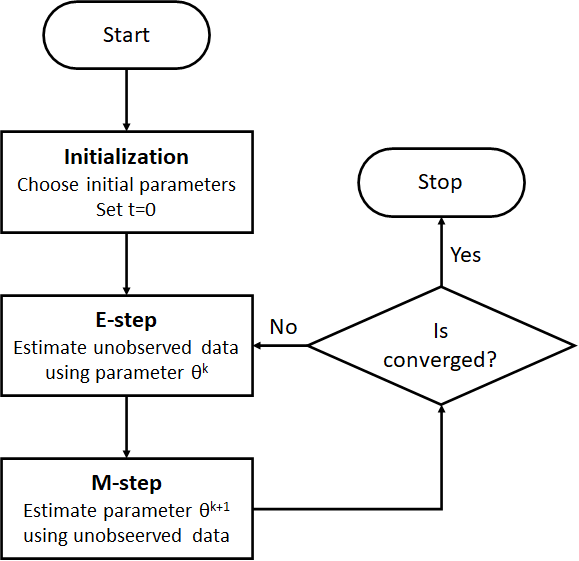
\includegraphics[width=9cm]{Part 3 - Learning Systems/Unsupervised Learning/Expectation-Maximization/figures/algorithm.png}
\caption{Flow chart for EM algorithm.}
\label{EM-algorithm}
\end{figure}

These two main steps are executed until the convergence of algorithm. The convergence is achieved when: the number of iterations (variable $t$ in the figure) equals to maximum number of iterations; there is no more difference between the actual partition and the previous one; or the difference of value of likelihood function for the actual partition and the value of likelihood function for the previous partition is below to some \textit{a priori} threshold.

\section{Applications}
\label{sec:applications}

Due to importance of the EM algorithm for Machine Learning, several researchers have been studying to apply this algorithm in an wide variety of real problems. These problems concern about Natural Language Processing, Signal Processing, medical image reconstruction and so on. This section shows some studies that applied EM algorithm as solution of real problems.

Ramme et al. (2009) \cite{ramme2009semi} used the EM algorithm to segment the hand phalanx bones. The goal of this work is to  analyze whether semi-automated technique will improve the efficiency while providing similar definitions as compared to a manual rater. %Figure \ref{EM-bone} shows surface models of the anterior aspects of the 12 phalanx bones after using EM algorithm.

%\begin{figure}[ht]
%\centering
%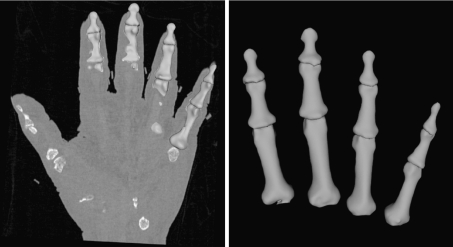
\includegraphics[width=8cm]{Part 3 - Learning Systems/Unsupervised Learning/Expectation-Maximization/figures/EM_bone.png}
%\caption{Computed Tomography image of the hand (left) and the posterior aspects of the bone models pictured alone (right) (from \cite{ramme2009semi}).}
%\label{EM-bone}
%\end{figure}

Kujawinska et al. (2016) \cite{kujawinska2016} applied EM algorithm to support purchasing decisions in the welding industry. Authors analyzed the EM for the selection of material (212 combinations of flux and wire melt) for the SAW (Submerged Arc Welding) method process. The work showed that each of the
212 records can be assigned with a probability of affiliation to all the four clusters used in the experiments. These probabilities allow the user make a better decision, since cases with ambiguous assignment can be better analyzed.

Subudhi et al. (2020) \cite{subudhi2020automated} used Expectation-Maximization and Random Forest classifier for automated segmentation and classification of brain stroke. The affected part of the brain due to stroke was segmented using EM algorithm and Magnetic Resonance Imaging (MRI) of brains. %Figure \ref{EM-MRI} shows the application of EM algorithm in the process of brain lesion detection.

%\begin{figure}[ht]
%\centering
%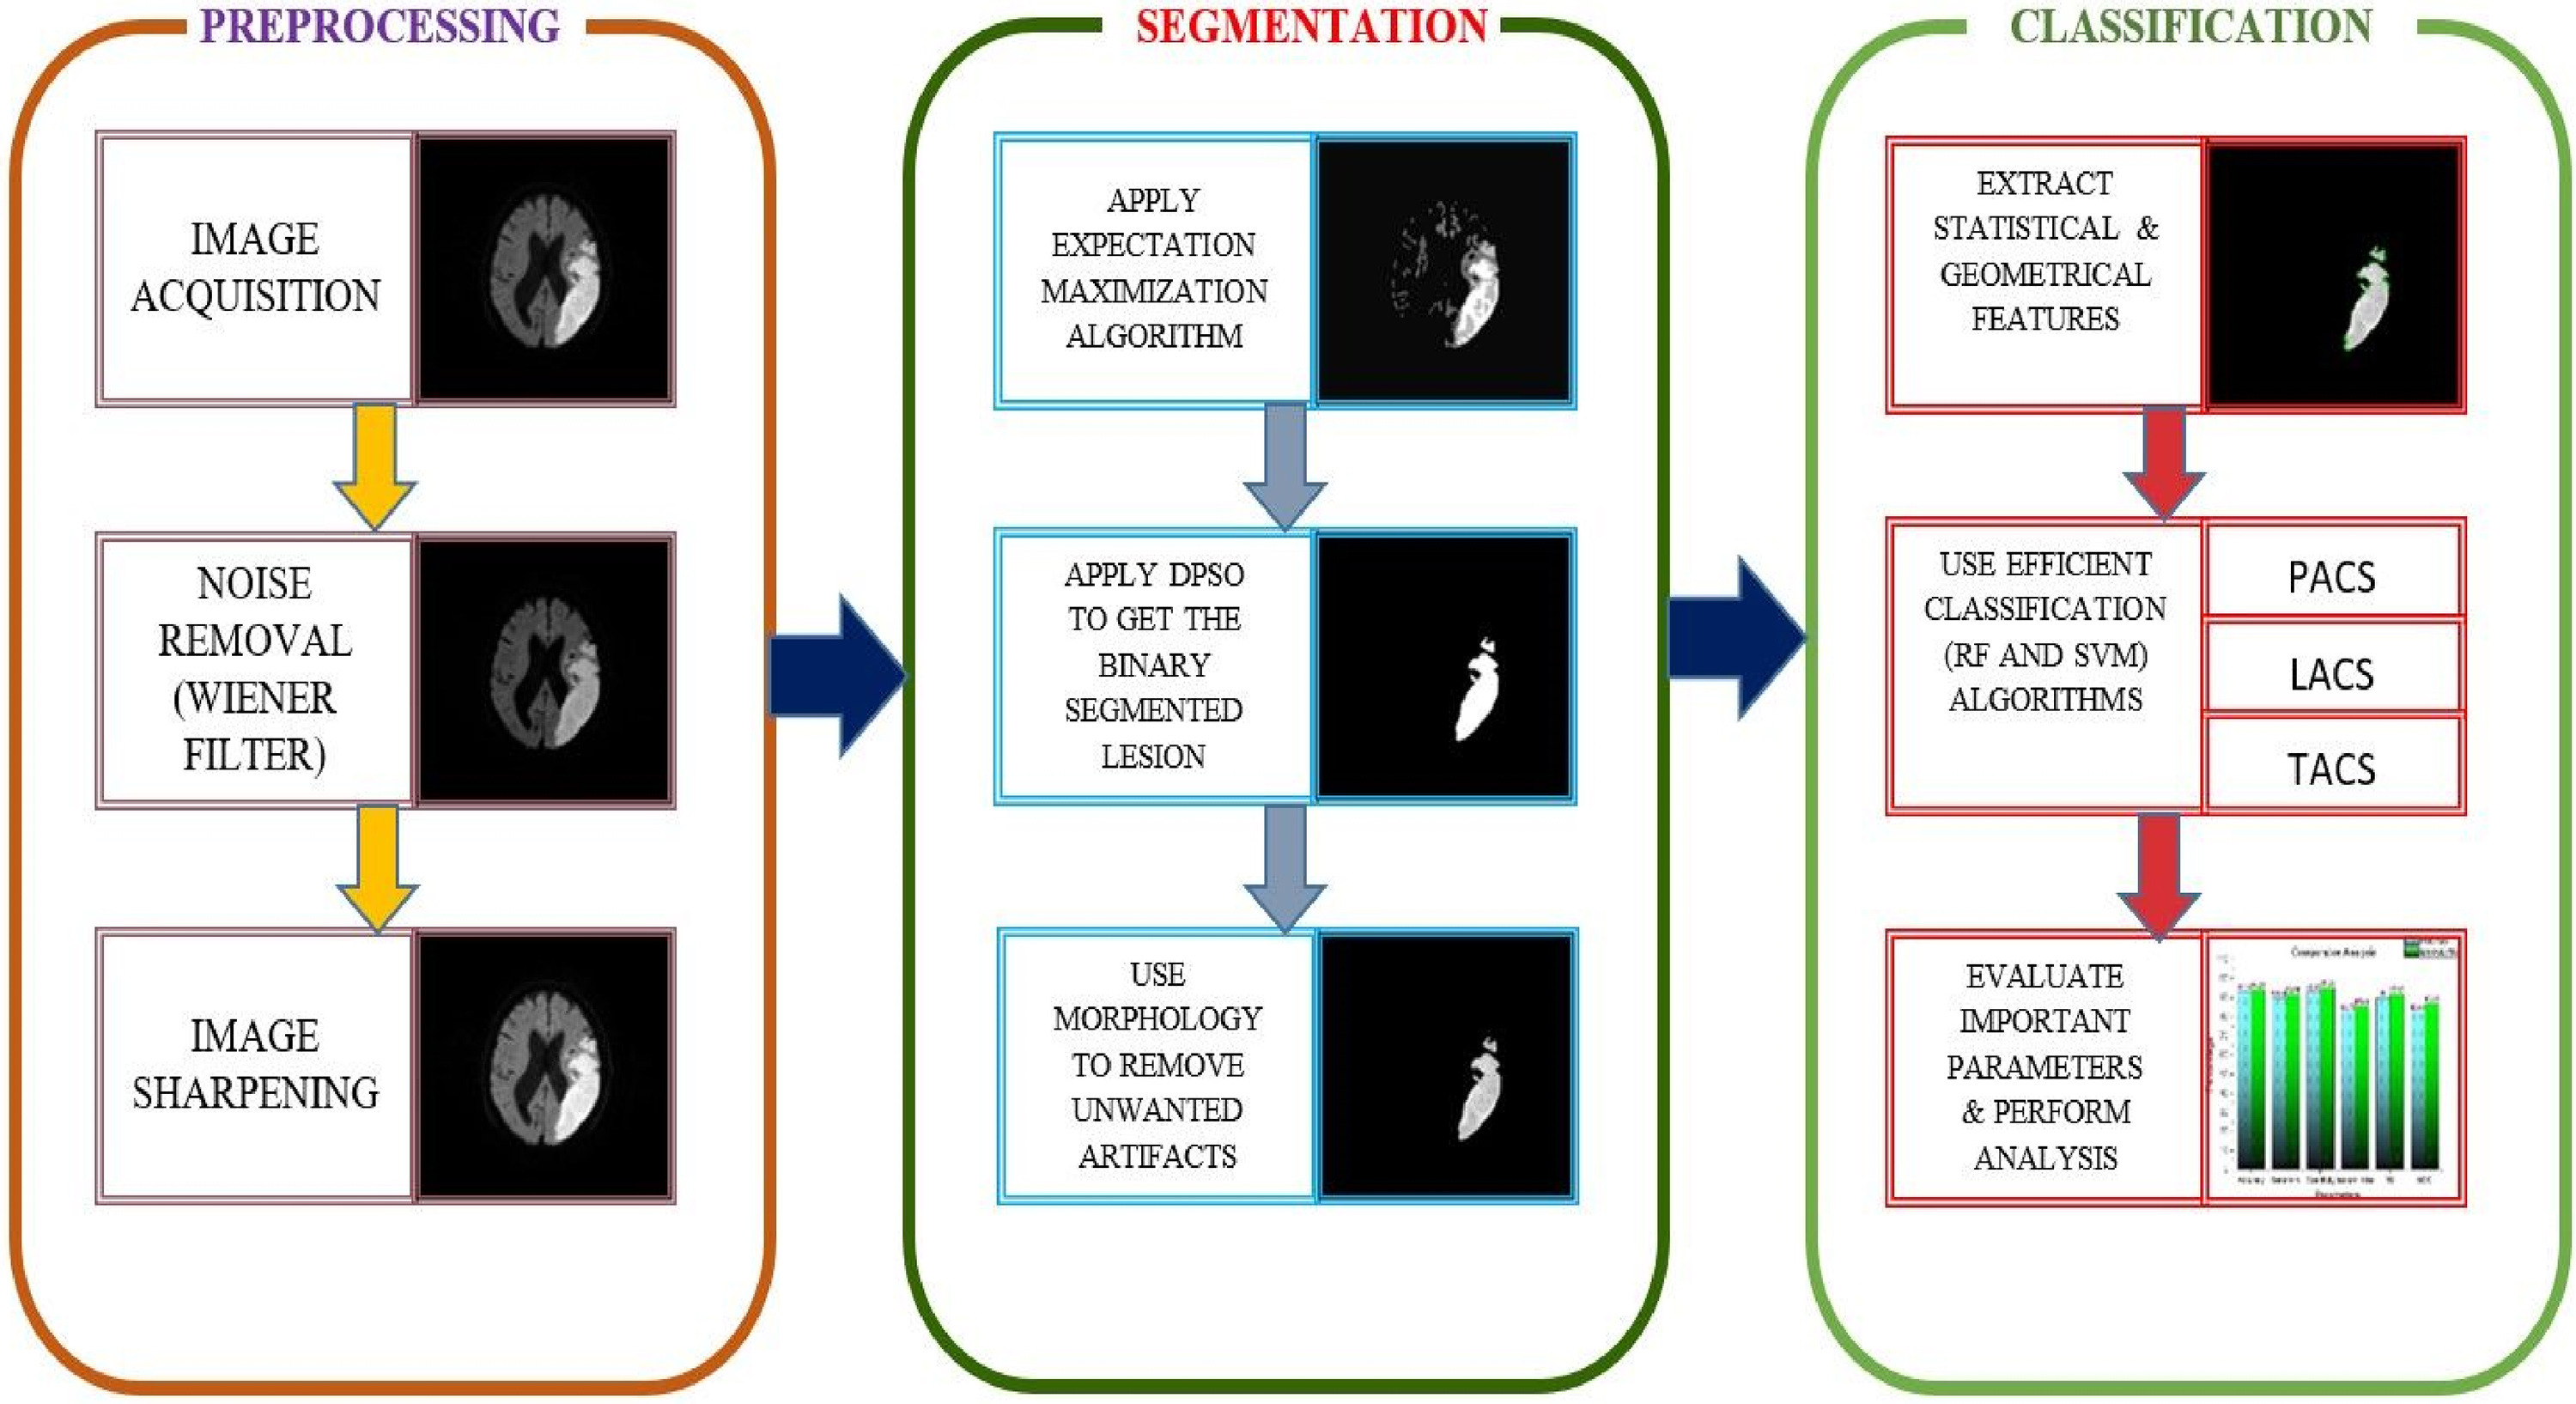
\includegraphics[width=10cm]{Part 3 - Learning Systems/Unsupervised Learning/Expectation-Maximization/figures/EM-MRI.png}
%\caption{Illustration of EM based method for lesion detection using MRI image (from %\cite{subudhi2020automated}).}
%\label{EM-MRI}
%\end{figure}

Lakshminarayanan et al. (2020) \cite{lakshminarayanan2020new} recovered the high-resolution image of a corresponding low-resolution image. For this, the paper proposed a new integrated approach based on the iterative super-resolution algorithm and EM for face hallucination (the process of improving a low resolution -- LR -- image to a high resolution -- HR -- image without altering the originality of the image). %Figure \ref{EM-image} shows the global face model learning.

%\begin{figure}[ht]
%\centering
%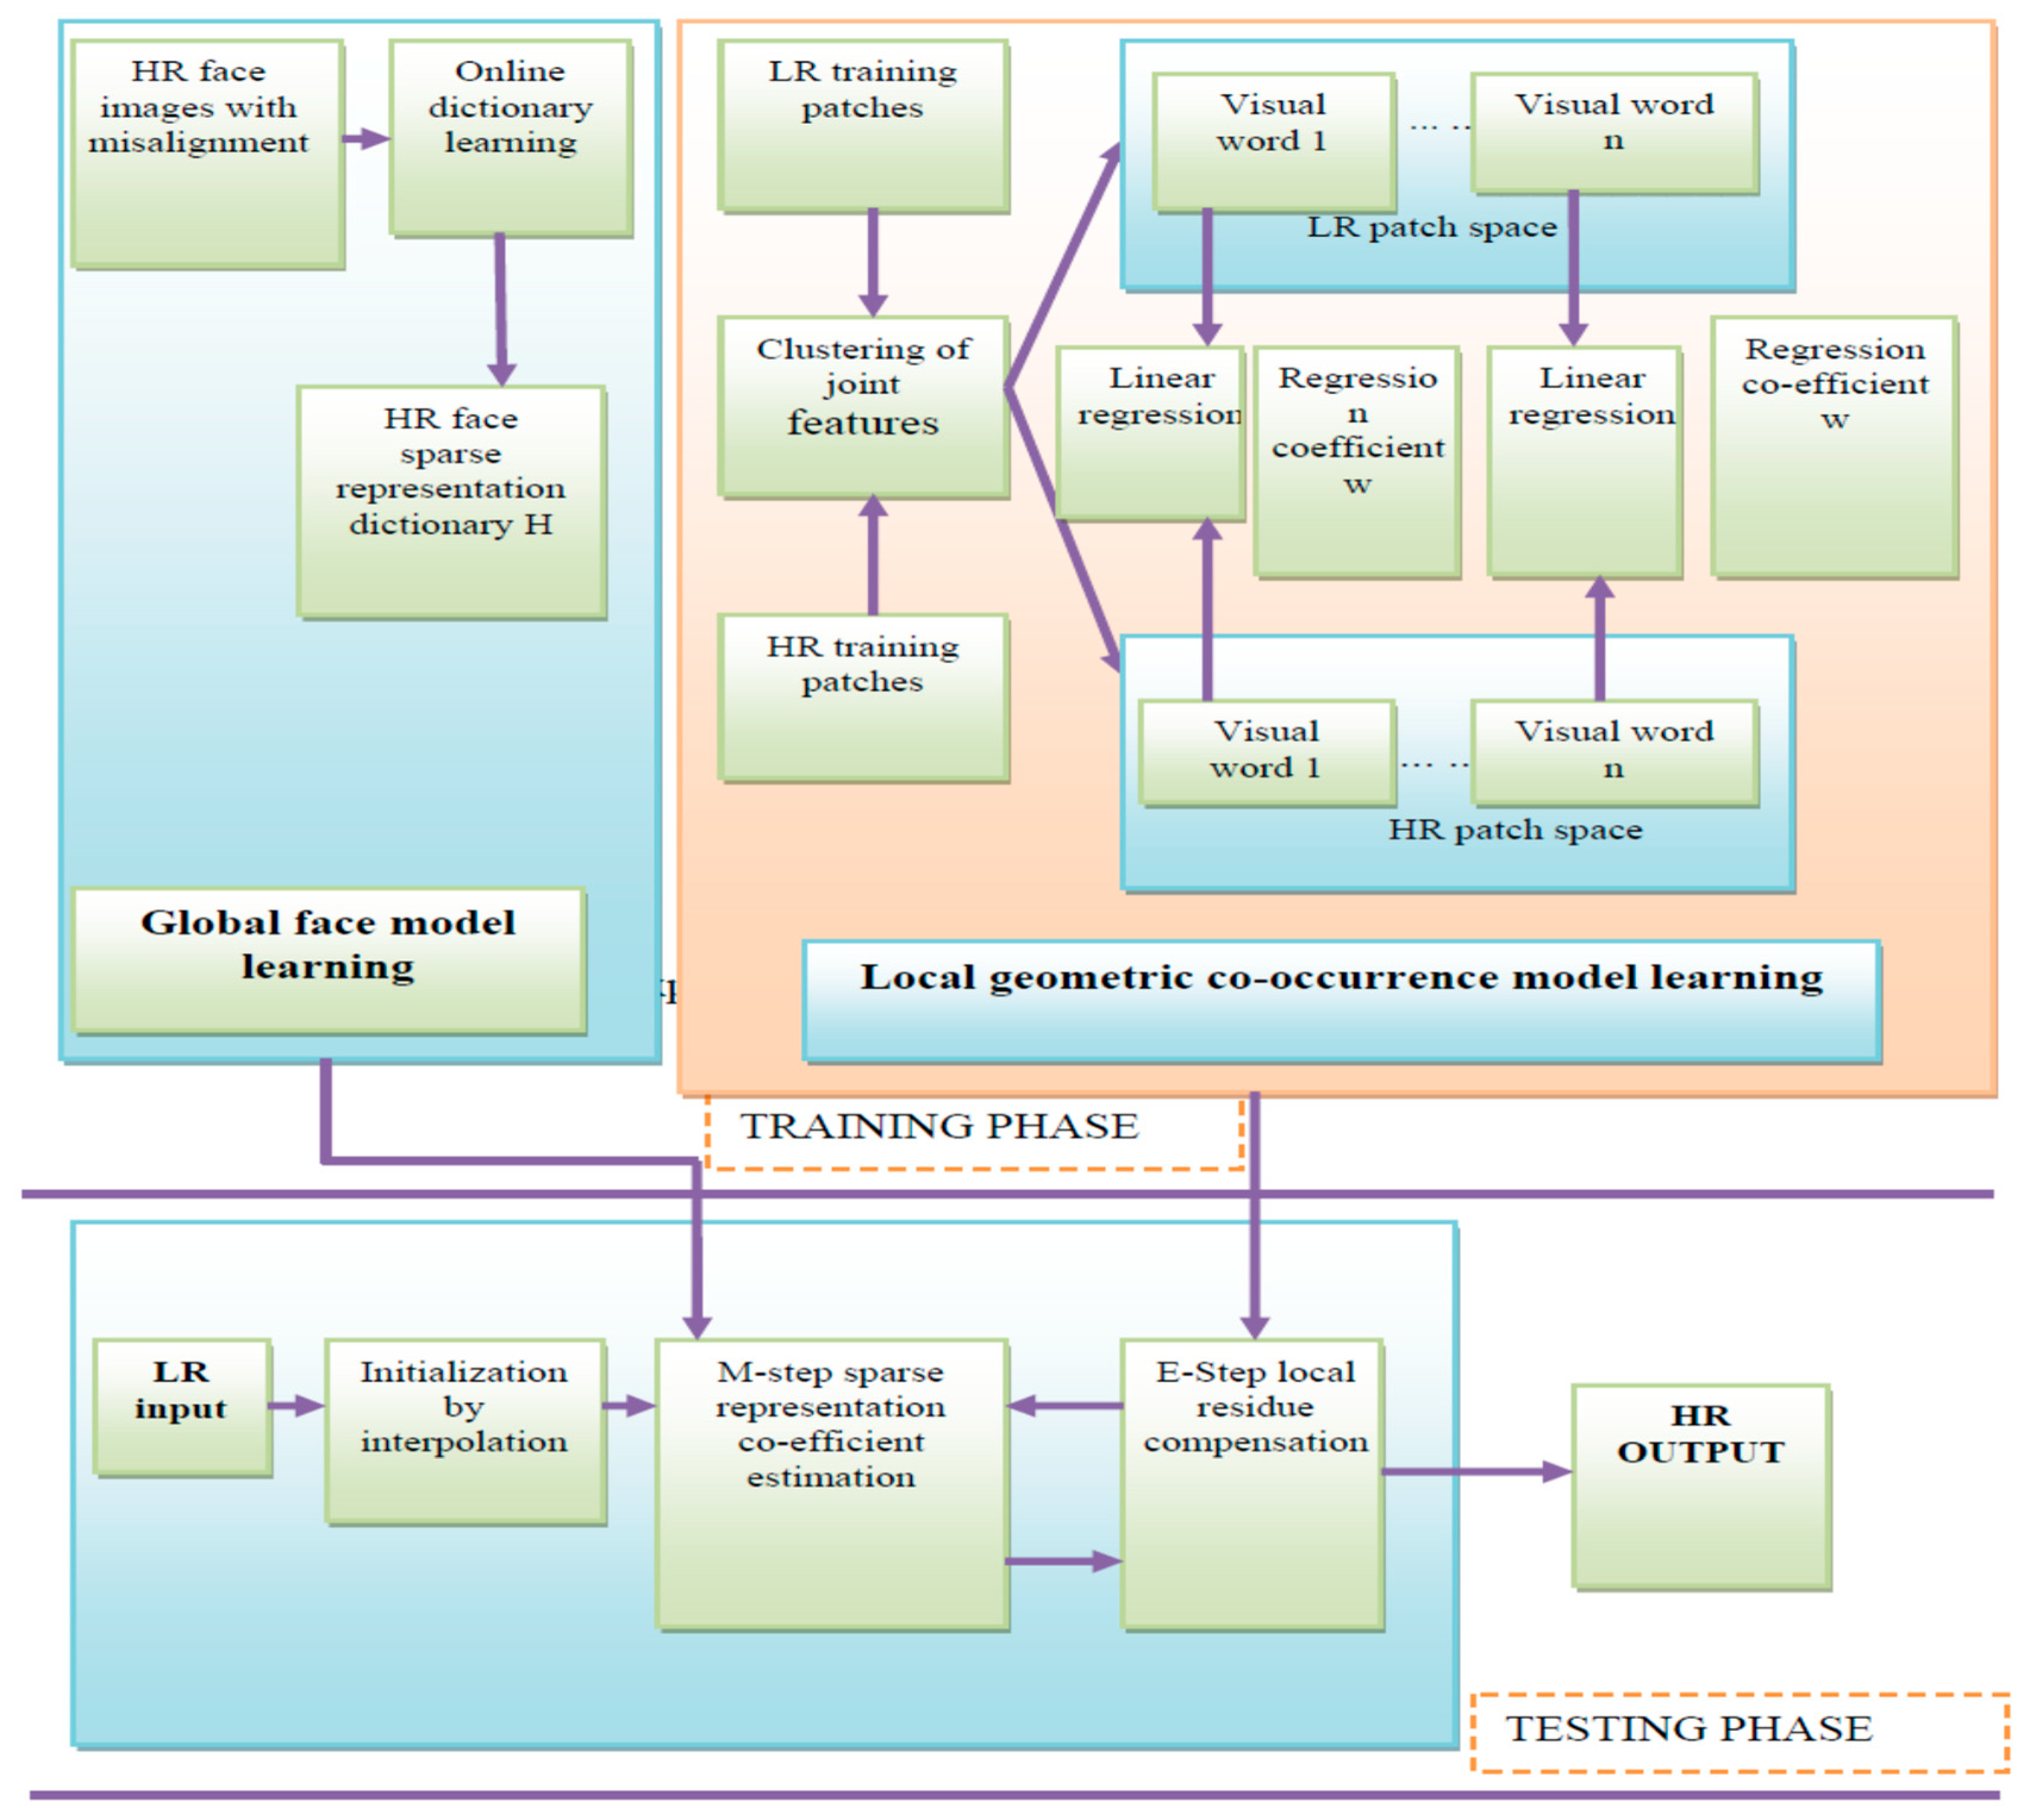
\includegraphics[width=10cm]{Part 3 - Learning Systems/Unsupervised Learning/Expectation-Maximization/figures/EM-image.png}
%\caption{Overview of model learning for the proposed approach (from %\cite{lakshminarayanan2020new}).}
%\label{EM-image}
%\end{figure}

\section{Exercises}

\begin{enumerate}
    \item Based on the experiment presented in Section \ref{sec:coin}, use EM algorithm to estimate the bias of each coin after 100 iterations.
    \item Use 300 samples of Gaussian Mixture with mixing probability equal to 1/3 as follow:
    \begin{equation*}
        X_1 \sim N\left( \begin{bmatrix} 1 \\ 1 \end{bmatrix}, \begin{bmatrix} 1 & 4 \\ 4 & 1 \end{bmatrix} \right)
    \end{equation*}
    
    \begin{equation*}
        X_2 \sim N\left( \begin{bmatrix} 5 \\ 5 \end{bmatrix}, \begin{bmatrix} 4 & 2 \\ 2 & 6 \end{bmatrix} \right)
    \end{equation*}
    
    \noindent and implements the EM algorithm to estimate its parameters.
    
    \item Show a scatter plot of the above dataset for different values of mixing probability: 1/2, 1/3, 1/4 and 1/5. What can you observe from the results?
    
    \item Changing the dataset to:
    
    \begin{equation*}
        X_1 \sim N\left( \begin{bmatrix} 1 \\ 1 \end{bmatrix}, \begin{bmatrix} 1 & 4 \\ 4 & 1 \end{bmatrix} \right)
    \end{equation*}
    
    \begin{equation*}
        X_2 \sim N\left( \begin{bmatrix} 5 \\ 5 \end{bmatrix}, \begin{bmatrix} 4 & 2 \\ 2 & 6 \end{bmatrix} \right)
    \end{equation*}
    
    \begin{equation*}
        X_3 \sim N\left( \begin{bmatrix} 3 \\ 3 \end{bmatrix}, \begin{bmatrix} 1 & 1 \\ 1 & 1 \end{bmatrix} \right)
    \end{equation*}
    
    \noindent repeat the question 3. What can you observe from the new results?
    
\end{enumerate}

\bibliographystyle{unsrt}
\bibliography{bibliography}